\subsection{Effizienz der Anwendung} \label{sec:application_efficiency}

Für die Überprüfung der Effizienz wurden der Server und der Client auf dem gleichen System betrieben.
Dabei wurde eine leere Welt mit einem Agenten kombiniert, der Fahrzeuge nach einem festen Muster bewegt.

Dieser Agent soll ganz gezielt so wenig wie möglich Zeit benötigen, da der Fokus hier auf den restlichen Komponenten liegt.

Die Messung wurde mit dem Chrome Browser Version 100.0.4896.75 und der Node.js Runtime Version v16.13.1 durchgeführt.
Die Anwendung wurde auf einem Computer mit einer Nvidia GForce 1060 3 GB, einem AMD FX 8320 8-Kern Prozessor und 32 GB RAM betrieben.
Als Betriebssystem diente Windows 10 Version 19044.

Der Agent wurde nun gestartet und für 10 Sekunden betrieben, dabei bewegt dieser abhängig vom aktuellen Frame die Fahrzeuge in einem Wellenmuster.
Vier Komponenten wurden dann gezielt mit Messpunkten versehen.
Diese Komponenten sind die, deren Laufzeit von der Anzahl der Fahrzeuge abhängt.

Diese Komponenten stellen die zentrale Abfolge aus \textit{Rendering} (dem Render-Pipeline- und three.js-Schritt), \textit{Deserializing} (die Frontend seitige Umwandlung von Binärdaten in JavaScript-Objekte), \textit{Serializing} (die Umwandlung von JavaScript-Objekten zu einer Binärrepräsentation im Worker) und schließlich dem \textit{Step} (die Erzeugung eines neuen Frames durch den Agenten) dar, die für jeden Frame durchlaufen werden muss.

\begin{table}[h!]
    \footnotesize{
        \makebox[\textwidth][c]{
            \begin{tabular}{ |r|r|r|r|r|r|r|r|r|  }
                \hline
                \multirow[b]{3}{4em}{Fahrzeuge} & \multicolumn{4}{c|}{Client Realm} & \multicolumn{4}{c|}{Agent Worker Realm} \\
                \cline{2-9}
                & \multicolumn{2}{c|}{Rendering} & \multicolumn{2}{c|}{Deserializing} & \multicolumn{2}{c|}{Serializing} & \multicolumn{2}{c|}{Step} \\
                \cline{2-9}
                & Time    & Rate       & Time    & Rate       & Time    & Rate       & Time   & Rate        \\
                \hline
                256    & 0,63ms  & 1.585,20Hz & 0,21ms  & 4.660,19Hz & 0,47ms  & 2.150,11Hz & 0,03ms & 29.408,88Hz \\ % real 53 hz im frontend, 56Hz im Backend
                512    & 0,75ms  & 1.325,23Hz & 0,39ms  & 2.561,37Hz & 0,82ms  & 1.215,89Hz & 0,04ms & 25.365,15Hz \\ % 52 real, 56 Backend
                1.024  & 0,99ms  & 1.010,10Hz & 0,79ms  & 1.273,21Hz & 1,19ms  & 840,96Hz   & 0,05ms & 20.244,45Hz \\ % 51 real, 56 Backend
                2.048  & 1,38ms  & 726,39Hz   & 1,47ms  & 678,16Hz   & 2,47ms  & 404,14Hz   & 0,21ms & 4.671,12Hz  \\
                4.096  & 2,86ms  & 349,96Hz   & 3,43ms  & 291,16Hz   & 4,56ms  & 219,22Hz   & 0,48ms & 2.103,71Hz  \\ % real 48, 54
                8.192  & 7,97ms  & 125,54Hz   & 9,46ms  & 105,68Hz   & 10,19ms & 98,16Hz    & 0,70ms & 1.435,29Hz  \\ % 36, 50
                16.384 & 14,27ms & 70,09Hz    & 20,51ms & 48,76Hz    & 27,20ms & 36,76Hz    & 0,73ms & 1.377,13Hz  \\ % 20, 28
                32.768 & 31,60ms & 31,65Hz    & 41,25ms & 24,24Hz    & 40,77ms & 24,53Hz    & 1,31ms & 766,04Hz    \\ % 10, 17
                \hline
            \end{tabular}
        }
    }
    \caption{Verarbeitungsgeschwindigkeitsmessung}
    \ownsource
    \label{table:2}
\end{table}

\textit{Time} ist die Zeit für einen Durchlauf der Komponente mit der jeweiligen Menge an Fahrzeugen und \textit{Rate} drückt dann das Inverse, also die mögliche Anzahl an Durchläufen pro Sekunde, aus.

Wie zu erkennen ist, beschränkt im stärksten Maße die (De-)Serialisierung.
Diese benötigt bei 32.768 Fahrzeugen auf beiden Seiten rund 40 ms womit die eigentlich Framerate sowohl bei der Erzeugung als auch bei der Darstellung auf 25Hz beschränkt ist.

Ein zusätzlicher Faktor sind die Datenmengen, die transportiert und dann im Speicher abgelegt werden müssen.
Bei 32.768 Fahrzeugen erreicht der Frame ein Volumen von 1.015.844 Bytes, die durch die Serialisierung erzeugt werden.
Das heißt bei 60 Hz müssten 60,95 MB pro Sekunde übertragen werden, womit mindestens eine Übertragungsrate von 488 MBit pro Sekunde benötigt werden würde.

Diese Datenraten erreicht man nur noch in ausreichend ausgestatteten lokalen Netzwerken, die eine Übertragungsrate von 500 MBit bzw. einem Gigabit zulassen.
Jedoch handelt es sich hierbei schon um eine sehr große Menge an Fahrzeugen.

Bei 4096 Fahrzeugen, was eine realitätsnähere Obergrenze sein sollte, sind das dann nur noch 61 Mbit pro Sekunde und bei 1024 Fahrzeugen 15 Mbit pro Sekunde.
Durch 1024 Fahrzeugen sollten schon viele Szenarien abdecken und einen großen Anteil an Wechselwirkungen erkennen lassen.
Durch die dafür benötigten 15 Mbit Up- bzw. Download ließen sich diese Simulationen dann sowohl über das Internet als auch im lokalen Netzwerk übertragen.

Größere Datenmengen erzeugen allerdings auch Probleme durch ihre Deserialisierung.

Bei 32.768 Fahrzeugen erhöht sich innerhalb 600 ms der allokierte Speicher im Browser, größtenteils durch die Deserialisierung, von 30 MB auf mehr als 130 MB, was dann eine Garbage Collection nach sich zieht.
Dadurch, dass diese den JS Thread blockiert, verringert sich der Anteil der Gesamtzeit, die das Script mit der Berechnung verbringt, auf nur noch etwa drei Viertel der real vergangenen Zeit.

\begin{figure}[htb]
    \centering
    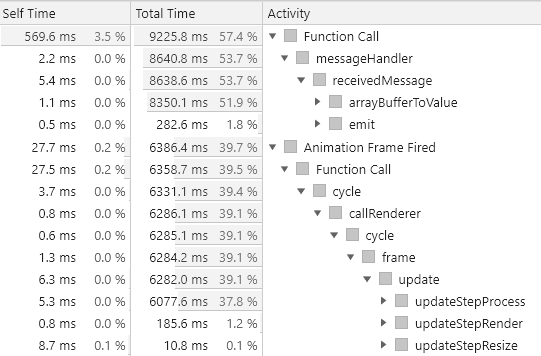
\includegraphics[scale=0.5,center]{medien/triss-perf.png}
    \caption{TRISS Performance Measurements}
    \ownsource
    \label{fig:triss-performance}
\end{figure}

Die eigentliche Pipeline nutzt von der gesamten JavaScript-Zeit etwa 37 \% (28 \% der realen Zeit), der eigentliche Pixel-Erzeugungsprozess durch WebGL ist nicht erfassbar.
Der Deserialize-Schritt braucht in etwa 52 \% (39 \% der realen Zeit) dieser Zeit.

In jedem Fall steht, vor allem im Bereich unter 4096 Fahrzeugen, serverseitig mit 70 \% der Zeit noch ein bedeutender Anteil der Rechenleistung für den Agenten bereit und das selbst dann, wenn man bei diesem einen Worker bleibt.
Die Implementation des Agenten könnte ebenso gut auf mehrere Worker verteilt werden, wodurch dann die restlichen Kerne ausgelastet werden könnten.
Mit 4096 Fahrzeugen sollten sich allerdings schon sehr viele unterschiedliche Szenarien abdecken und simulieren lassen.

Somit wirkt diese Implementation mit dem JavaScript-Ökosystem nicht als \enquote{Flaschenhals} und steht damit selbst bei aufwendigeren Szenarien dem Agenten nicht im Weg.
